\chapter{\label{ch:experiments}Experiments}
In this chapter, we will describe the experiments we made and present the
results we obtained. In Section~\ref{sec:clone-detection-experiments}, we will
present our experiments about code clone detection, while in
Section~\ref{sec:token-generation-experiments} we will describe our experiments
to generate token embedding. In both sections we will show what kind of data we
used to train our model and how our model perform with different
hyper-parameters.
\section{\label{sec:clone-detection-experiments}Code clone detection}
To evaluate our clone detection model, we implemented the model we described
in~\ref{sec:clone-detection}, we collected data of programs implementing the
same functionality to feed to the model, and we trained and evaluated our model
with different hyper-parameters. In this section, we will give some details
about the data we collected for our experiments and present the different
results we obtained when evaluating our model.
\subsection{\label{ssec:clone-detection-dataset}Code clone detection dataset}
As we are using a supervised learning approach to code clone detection, to train
our model we needed data which fulfills the following properties.

\begin{enumerate}
\item Multiple code fragments should implement the same functionality
\item Information on whether two code fragments implement the same functionality
  must be included
\item Dataset should contain code fragments written in at least 2 programming
  languages
\end{enumerate}

To the best of our knowledge, no dataset currently available fulfills all the
necessary properties to our experiments, therefore we created our own dataset.

For this dataset, we found that competitive programming websites are an
excellent match. The solution to a single problem is implemented by a
large number of persons in many different languages. All the solutions to a
single problem must implement exactly the same functionality, therefore,
we are assured that all source codes implementing a solution to the same problem
are at least type IV code clones. The easier the problem is, the higher the
probability of code fragments implementing the solution to the same problem have
to be very similar to each other, and to therefore be closer to type III clones.
Furthermore, multiple solutions to a problem are always implemented by different
users, which makes our dataset closer to the motivating example we presented in
Section~\ref{sec:motivating-exmaple}.

To create the dataset, we scraped code from a famous Japanese competitive
programming website. As our implementation currently only supports Java and
Python, we fetched data for these two programming languages. We restricted the
data to only programs that were accepted by the website judging system --- meaning
that the programs actually implemented the solution to the given problem --- in
order to have the type IV code clone guarantee. In
table~\ref{tab:clone-dataset-overview}, we give some statistics about the
dataset we created and in table~\ref{tab:clone-dataset-languages} we show how
the given statistics are distributed between Python and Java. We show the
distribution of the number of files per problem --- which is representative of
the number of clones in the dataset --- in
figure~\ref{fig:files-per-problem-distribution}.

\begin{table}
  \caption{\label{tab:clone-dataset-overview} Clone detection dataset overview}
  \begin{center}
    \begin{tabular}{c c}
      Measure & Value\\
      \toprule
      Problems count & 576\\
      Avg. files / problem & 77\\
      Files count & 44620\\
      Lines count & 1270599\\
      Tokens count & 8554476
    \end{tabular}
  \end{center}
\end{table}

\begin{table}
  \caption{\label{tab:clone-dataset-languages} Clone detection dataset language overview}
  \begin{center}
    \begin{tabular}{c c c}
      & Python & Java\\
      \toprule
      Avg. files / problem & 41 & 36\\
      Files count & 23792 & 20828\\
      Lines count & 312353 & 958246\\
      Tokens count & 1810085 & 6744391
    \end{tabular}
  \end{center}
\end{table}

\begin{figure}
  \begin{center}
    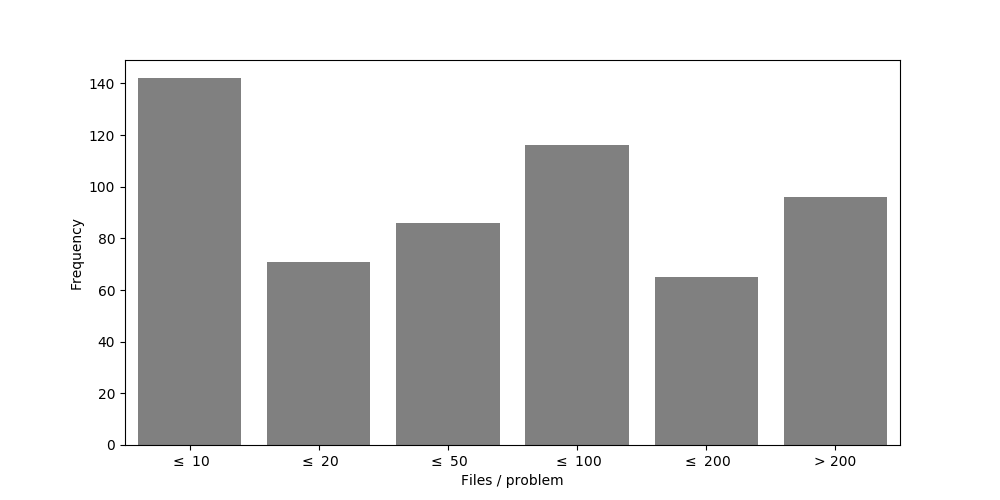
\includegraphics[width=16cm]{./images/code-clone-dataset-problems-distribution.png}
    \caption{\label{fig:files-per-problem-distribution} Distribution of the
      number of files per problem}
  \end{center}
\end{figure}

In order to be able to feed the code to our model, we transform the code we
fetched using \lstinline{bigcode-astgen} we presented in
Section~\ref{sec:ast-generation} using the commands shown in
listing~\ref{lis:atcoder-astgen}.

\begin{lstlisting}[numbers=none,language={},
  caption=AST generation using \lstinline{bigcode-astgen}, label=lis:atcoder-astgen]
bigcode-astgen-java --batch -f 'src/**/*.java' -o java-asts
bigcode-astgen-py --batch -f 'src/**/*.py' -o python-asts
cat java-asts.json python-asts.json > asts.json
cat java-asts.txt python-asts.txt > asts.txt
\end{lstlisting}
With the first two commands, we generate the ASTs for Python and Java source
files, and with the next we commands we merge the ASTs and the file which maps
the index of the AST in the JSON file to the name of the file in the original
dataset.
\subsection{\label{ssec:clone-detection-hyper-params}Code clone detection model hyper-parameters}
Our model contains many hyper-parameters that can vastly influence its
performances while detecting clones. In listing~\ref{lis:model-config}, we show a
sample configuration file that we actually use to train our model.

\begin{figure}
  \lstinputlisting[language={}, basicstyle=\ttfamily\footnotesize, caption=Model
  configuration file,label=lis:model-config]{./snippets/config.yml}
\end{figure}

We will describe the meaning of each parameter in our configuration file.

\begin{description}
\item[{\small\texttt{transformer\_class\_name}}] The algorithm to used to encode
  the AST into a vector as described in~\ref{sssec:ast-transformer}
\item[{\small\texttt{vocabulary}}] The path to the extracted vocabulary
\item[{\small\texttt{embeddings}}] The path to the trained token embedding. If
  this parameter is not provided, embedding are randomly initialized
\item[{\small\texttt{embeddings\_dimension}}] The dimension $d_w$ of the trained embedding
  for the target programming language as described in~\ref{sssec:token-embedding-layer}
\item[{\small\texttt{output\_dimensions}}] The output dimension $d_e$ of the
  LSTM encoder described in~\ref{sssec:lstm-encoder}. If the length of the array
  is greater than $1$, the LSTM will be stacked and the output dimension will be
  the value of the last element of the list
\item[{\small\texttt{bidirectional\_encoding}}] Whether or not to use a
  bidirectional LSTM
\item[{\small\texttt{name}}] The name of the programming language
\item[{\small\texttt{input\_length}}] The maximum number of tokens per code
  fragment. This restriction can be avoided at the cost of a performance penalty
\item[{\small\texttt{merge\_mode}}] The algorithm to use to merge the two code
  fragments as described in~\ref{sssec:merge-layer}
\item[{\small\texttt{merge\_output\_dim}}]The output dimension to use for the merge layer. Currently only effective
  when using equation~\ref{eq:bidistance-merge-layer} as the merge layer
\item[{\small\texttt{dense\_layers}}] The number of hidden layers to use for the
  final MLP and their number of units
\item[{\small\texttt{optimizer}}] The optimizer to use to train the model
\item[{\small\texttt{submissions\_path}}]The path of the training dataset
  submissions metadata
\item[{\small\texttt{asts\_path}}] The path of the training data ASTs generated
  as described above
\item[{\small\texttt{split\_ratio}}] The amount of data to use for training,
  hyper-parameter tuning, and testing the model
\item[{\small\texttt{shuffle}}] Whether or not to shuffle the data when training
  the model
\item[{\small\texttt{negative\_samples}}] The number of non-clone noise data ---
  negative sample --- to generate per code clone
\item[{\small\texttt{negative\_sample\_distance}}] The maximum distance ratio
  between the size of the input and the size of the negative sample, to avoid
  the model to try to detect clones by number of tokens
\item[{\small\texttt{class\_weights}}] The weight to assign to positive and
  negative samples. The higher the weight, the more an error will be penalized
\item[{\small\texttt{batch\_size}}] The size of a batch when training the model
\item[{\small\texttt{epochs}}] The number of epochs for which to train the model
\end{description}
\section{\label{sec:token-generation-experiments}Token embedding generation}
